\documentclass[12pt]{article}
\usepackage[document]{ragged2e}
\usepackage{mathptmx} %Times New Roman Font%
\usepackage[a4paper, margin=1 in]{geometry} % Ukuran Kertas A4 dan Margin 2.5cm pada setiap sisi %
\vspace{1.15cm} % Spasi 1.15 %
\usepackage{listings}
\usepackage{hyperref}
\hypersetup{
    colorlinks=true,
    linkcolor=blue,
    filecolor=blue,      
    urlcolor=blue,
    pdftitle={Overleaf Example},
    pdfpagemode=FullScreen,
    }

\usepackage{graphicx}
\graphicspath{ {./images/} }

\begin{document}
    % Title %
    \begin{center}
        Tugas Project Penelusuran Informasi 2023

        Diky Wahyudi (2108107010031)
    \end{center}

    \section*{Hasil Analisa Program Index-C}
    Pada tugas ini, diberikan sebuah program untuk melakukan index dalam bahasa C. Lalu dilakukan \textit{Debugging} dan melakukan perbaikan pada kode tersebut.

    \subsection*{Hasil analisa pada file keluaran dari program}
    Pada program dihasilkan 5 file keluaran yaitu
    \begin{itemize}
        \item \textbf{data.inv}
        \begin{flushleft}
            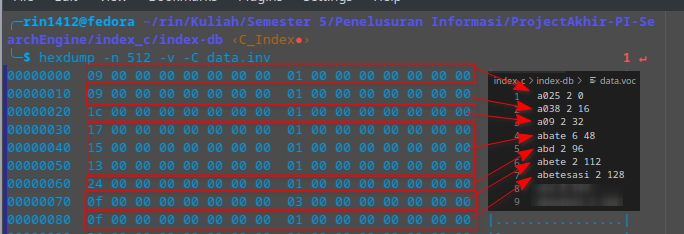
\includegraphics[scale=0.8]{images/index-1.png}
            
            \justifying
            Padafile \textbf{data.inv} berisikan nomor dokumen dan frekuensi dari sebuah kata dengan urutan sesuai dengan kata pada file data.voc

            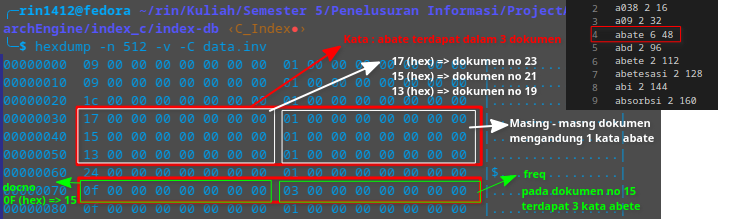
\includegraphics[scale=0.7]{images/index-2.png}

            \justifying
            Struktur dari data.inv untuk setiap data kata pada sebuah dokumen terdapat 2 nilai yaitu docno yaitu nomor dokumen dan freq yaitu jumlah kemunculan kata dalam dokumen tersebut. Kedua nilai ini disimpan dalam bentuk long int (32 bit) sehingga untuk setiap kemunculan kata dalam sebuah dokumen diperlukan 64 bit.
        \end{flushleft}

        \item \textbf{data.nme}
        \begin{flushleft}
            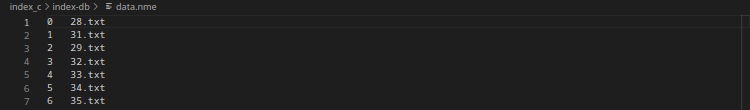
\includegraphics[scale=0.75]{images/nme.png}

            \justifying
            Pada file data.nme berisi daftar dari nomor dokumen dan nama file dari dokumen tersebut.
        \end{flushleft}
        
        \item \textbf{data.par}
        \begin{flushleft}
            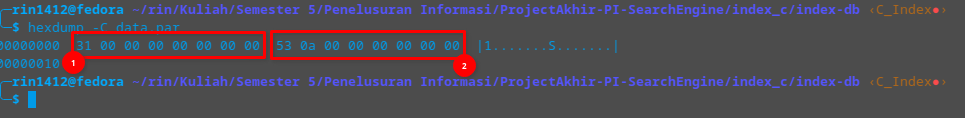
\includegraphics[scale=0.58]{images/param.png}

            \justifying
            Pada file data.par berisikan 2 buah parameter yaitu
            \begin{itemize}
                \item Banyak dokumen (Nomor 1) Dengan tipe long int (32bit)
                \item Banyak kata unik (Nomor 2) dengan tipe long int (32bit)
            \end{itemize}
        \end{flushleft}

        \item \textbf{data.voc}
        \begin{flushleft}
            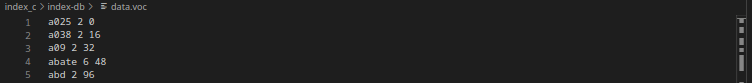
\includegraphics[scale=0.74]{images/voc.png}

            \justifying
            Pada file data.voc berisikan semua kata yang unik, jumlah kata dan offset (letak kata pada index data.inv dalam bytes)
        \end{flushleft}

        \item \textbf{data.wdl}
        \begin{flushleft}
            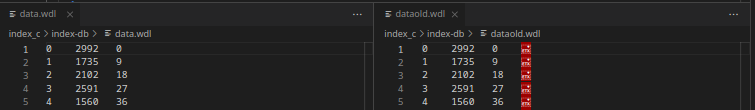
\includegraphics[scale=0.74]{images/wdl.png}

            \justifying
            Pada file wdl berisikan datkanana nomor dokumen, panjang dokumen dan nilai offset nomor dan nama dokumen yang terdapat pada file data.nme. Pada gambar kanan adalah file yang sebelum diperbaiki terdapat bagian yang error dikarenakan melakukan write sebuah variabel kosong. Gambar kiri adalah keadaan file ketika telah dilakukan perbaikan.
        \end{flushleft}
    \end{itemize}

    \subsection*{Debugging dan Perbaikan pada kode program}
    Setelah dilakukan \textit{Debugging} dan didapatkan sumber dari \textit{Bug} dilakukan perbaikan pada kode program. Berikut beberapa bagian yang telah dilakukan perbaikan

    \begin{itemize}
        \item \textbf{index-db.c}
        \begin{itemize}
            \item \textbf{Tidak dapat membuka file (kesalahan path)}
            \begin{flushleft}
                \justifying
                Penambahkan \textbf{strcat(path,"/")} untuk memperbaiki path.
            \end{flushleft}

            \item \textbf{Kesalahan ketika melakukan write kedalam file data.wdl}
            \begin{flushleft}
                \justifying
                Menghilangkan variabel \textbf{char class[WORDLEN]}, variabel ini tidak pernah diisi dan dilakukan write pada file data.wdl dan dilakukan perubahan dengan menghilangkan write variabel class. 
                Sebelumnya \textbf{fprintf(finf, "\%ld\t \%ld \t\%ld\t \%s\textbackslash n", docno, doclen, offset, class)} menjadi \textbf{fprintf(finf, "\%ld\t \%ld \t\%ld\textbackslash n", docno, doclen, offset)} sehingga file data.wdl hanya menyimpan docno, doclen, offset.
            \end{flushleft}
        \end{itemize}

        \item \textbf{define.h}
        \begin{itemize}
            \item \textbf{Nilai Buffer 256 terlalu kecil }
            \begin{flushleft}
                \justifying
                Terjadi warning ketika membaca file data.nme nilai yang dibaca adalah 512bytes sedangkan ukuran buffer hanya 256bytes. Nilai Buffer dinaikkan menjadi 512bytes
            \end{flushleft}
        \end{itemize}
        
        \item \textbf{query-with-doclen.c}
        \begin{itemize}
            \item \textbf{Bytes yang dibaca pada data.inv tidak sesuai dengan ukuran variabel penampung ilbuf}
            \begin{flushleft}
                \justifying
                Pada kode yang melakukan read pada file index \textbf{fread(ilbuf,sizeof(int),len,finv);} diubah menjadi \textbf{fread(ilbuf,sizeof(long int),len,finv);}
            \end{flushleft}

            \item \textbf{Kesalahan ketika melakukan normalisasi accumulator}
            \begin{flushleft}
                \justifying
                Pada kode untuk melakukan normalisasi nilai accumulator, nilai accumulatoor akan dibagi dengan panjang dokumen. Namun pada kode index panjang dokumen salah dan bernilai statis tidak. Sehingga prehitungan normalisasi menjadi salah dan pada kasus tertentu menyebabkan \textit{core dump} error.
                Pada bagian \textbf{accumulator[i] += accumulator[i] / fileinfo[docno].doclen;} di ubah menjadi \textbf{accumulator[i] += accumulator[i] / fileinfo[i].doclen;} Karena docno bukanlah variabel yang relevan dengan panjang setiap dokumen.
            \end{flushleft}
        \end{itemize}
        
        \item \textbf{Merubah isi stopword}
        \begin{itemize}
            \item \textbf{Merubah isi dari stoplist menjadi bahasa indonesia}
            \begin{flushleft}
                \justifying
                Ketika merubah isi stoplist, harus dilakukan update banyaknya stopword yang ada dalam stoplist pada file \textit{define.h}

                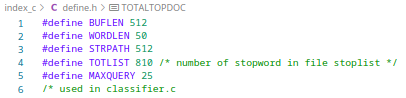
\includegraphics[scale=1.2]{images/sw.png}
            \end{flushleft}
        \end{itemize}
    \end{itemize}

    \section*{Pembangunan Aplikasi}
    Pada tugas ini akan dibangun sebuah \textit{Website - Search Engine} dengan menggunakan 3 \textit{tools} yaitu \textbf{Index-C, Apache Nutch+Solr, Swish-E} 

    \subsection*{Membangun Front-End Aplikasi}
    \justifying
    Pada bagian Front-End digunakan TailwindCSS sebagai \textit{Framework CSS}

    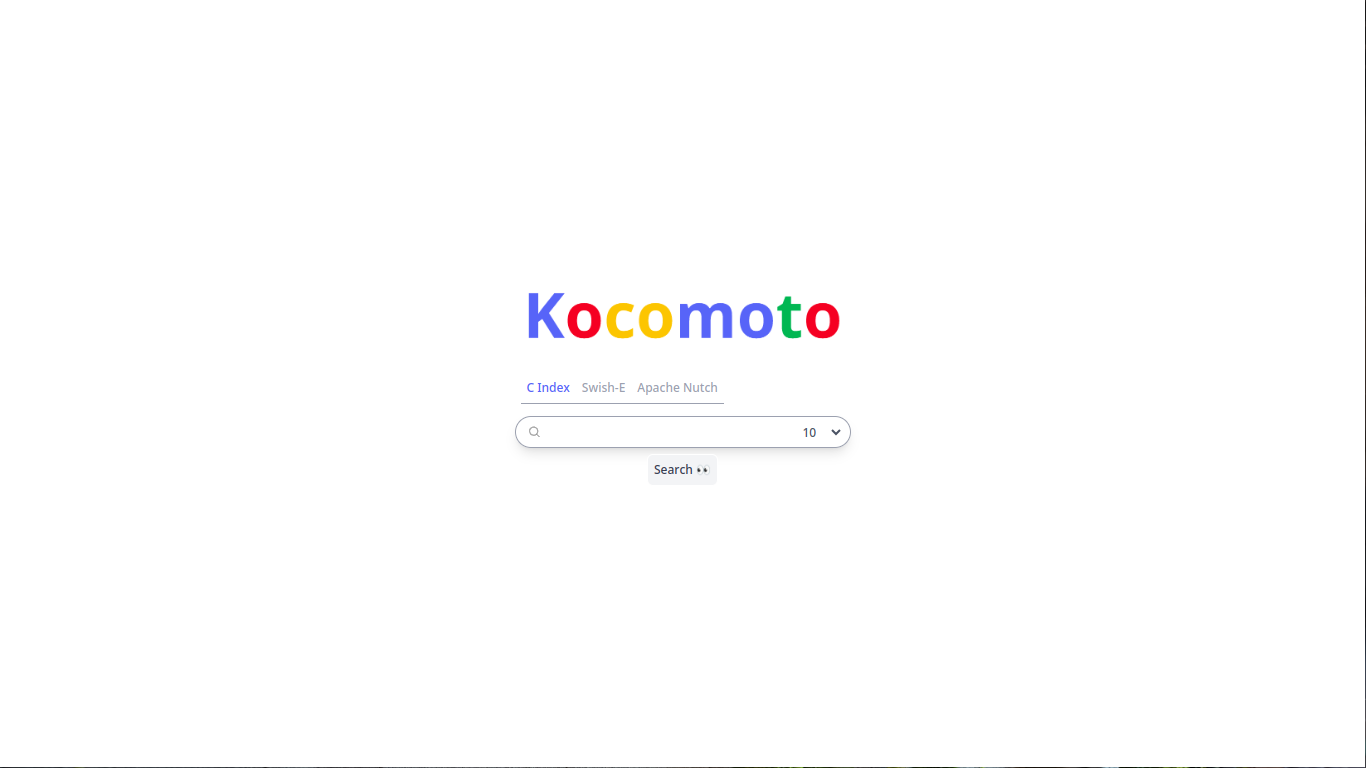
\includegraphics[scale=0.42]{images/mainpage.png} \newline
    \centering
    Halaman utama

    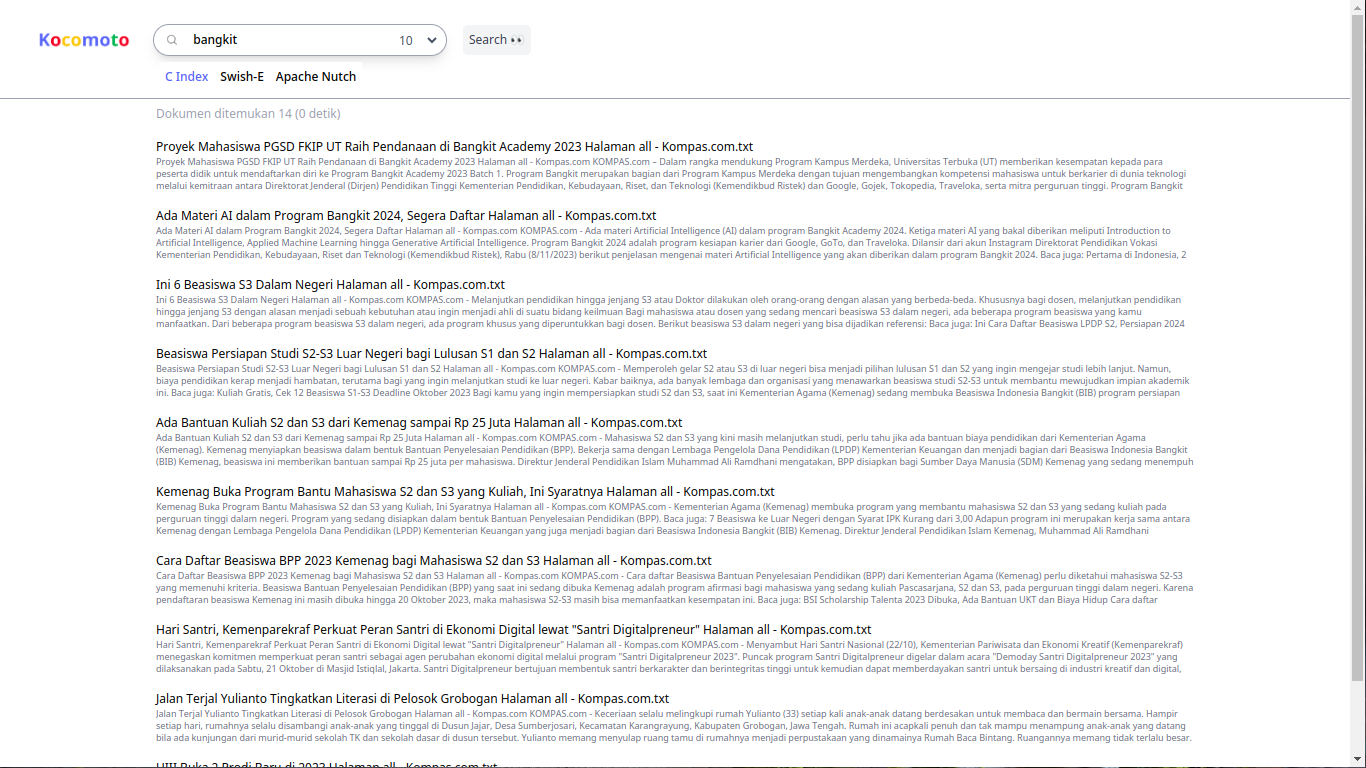
\includegraphics[scale=0.42]{images/searchpage.png} \newline
    Halaman Search

    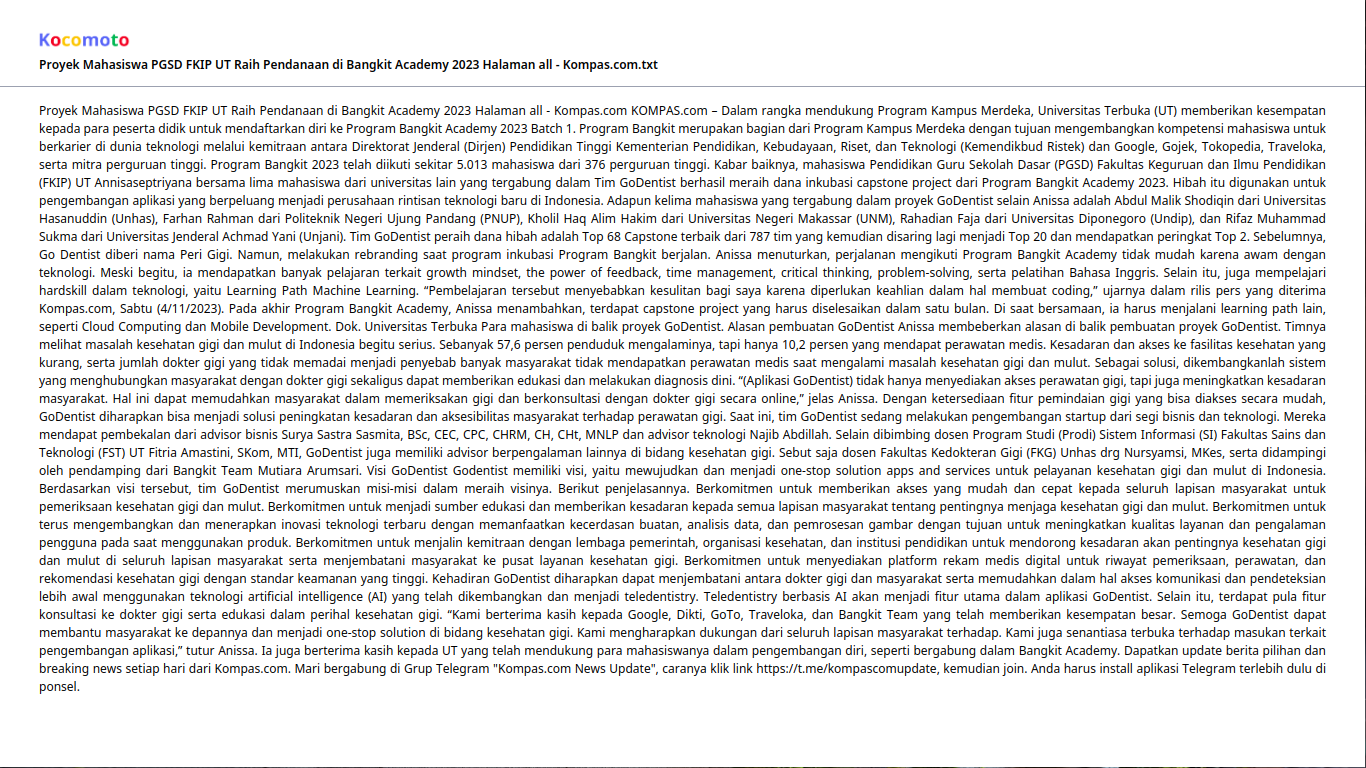
\includegraphics[scale=0.42]{images/openpage.png} \newline
    Halaman buka file

    \justifying
    \subsection*{Membangun Backend-End Aplikasi}
    Pada bagian Back-End digunakan Flask sebagai \textit{Framework Web}

    Kode Flask, terdapat 3 route yang dapat di akses yaitu HalamanUtama, HalamanSearch, dan HalamanBukaFile

    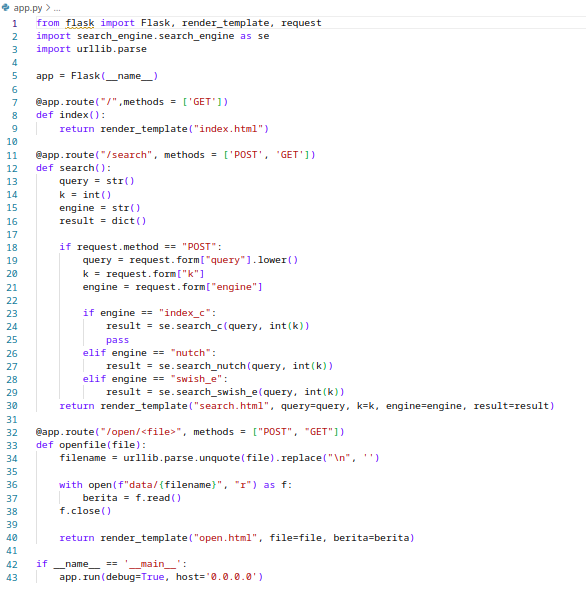
\includegraphics[scale=0.8]{images/appcode.png}

    Membuat sebuah module untuk membaca hasil output dari setiap engine index yang digunakan

    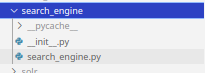
\includegraphics[scale=2.7]{images/module-se.png}

    Program C untuk membuat index dan melakukan query

    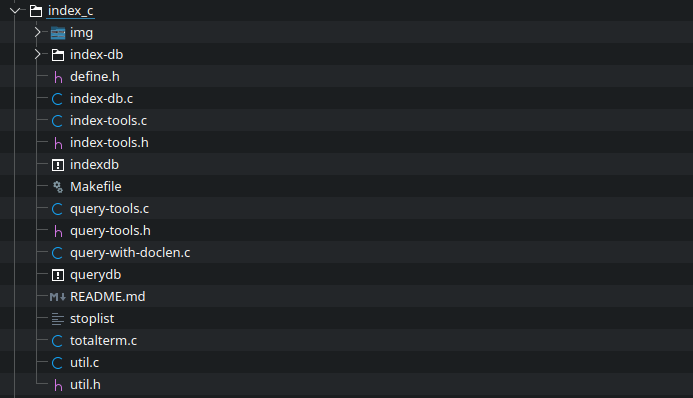
\includegraphics[scale=0.8]{images/c.png}
    
    Program Apache Solr untuk membuat index dan melakukan query

    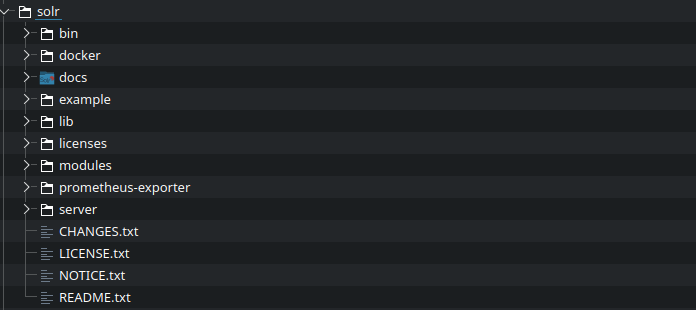
\includegraphics[scale=0.8]{images/solr.png}

    Program Swish-E untuk membuat index dan melakukan query

    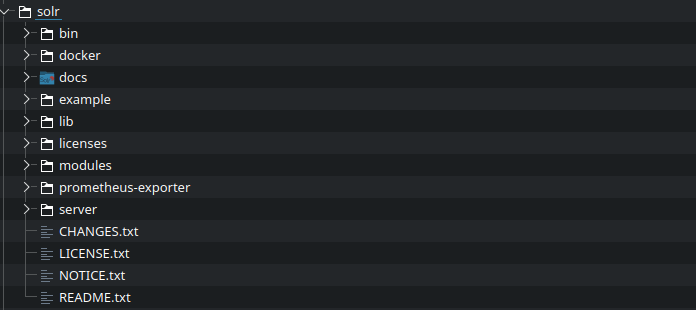
\includegraphics[scale=0.8]{images/solr.png}

    \subsection*{Membangun Script untuk melakukan Build pada project}

    Program \textit{Bash Script} untuk melakukan build pada program dengan nama \textbf{setup.sh}

    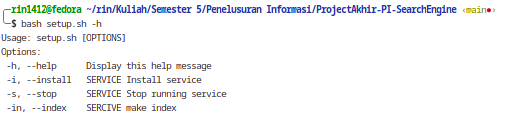
\includegraphics[scale=1.1]{images/script.png}
    
    \subsection*{Membangun Script Dockerfile untuk membuat docker image}
    Program \textit{Dockerfile} untuk menjalankan script pada container docker sehingga dapat membuat docker images dan dijalankan dengan menggunakan container docker
    
    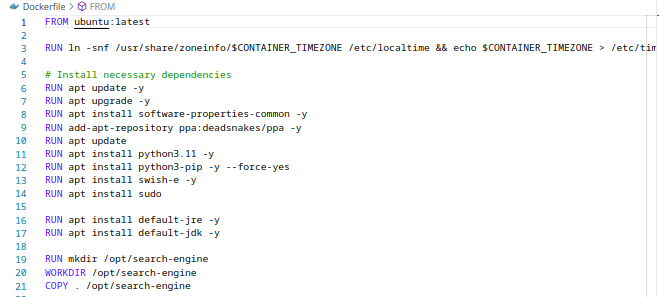
\includegraphics[scale=0.85]{images/docker.png}

    \newpage
    \section*{Hasil Query dan Perbandingan}

    Hasil query dari Index-C

    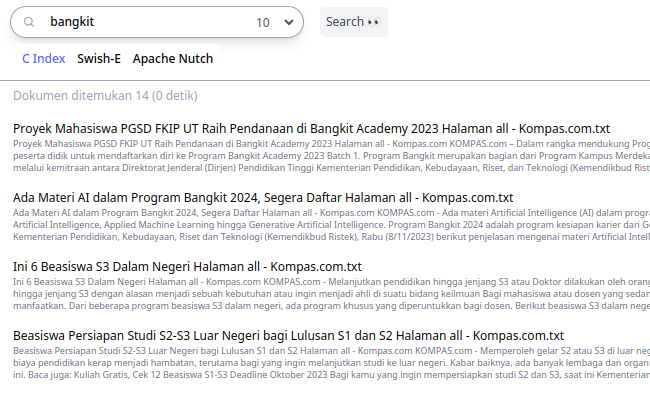
\includegraphics[scale=0.88]{images/query-c.png}

    Hasil query dari Swish-E

    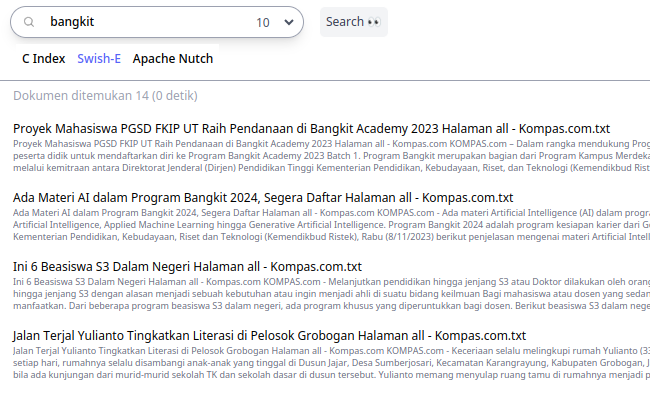
\includegraphics[scale=0.88]{images/query-swish.png}

    \newpage
    Hasil query dari Nutch

    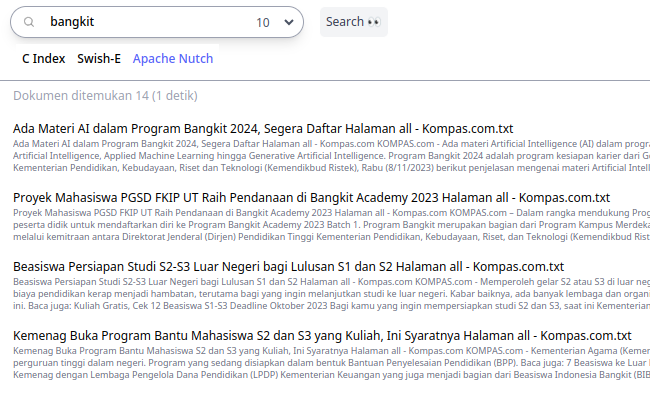
\includegraphics[scale=0.88]{images/query-nutch.png}

    \subsection*{Analisa Perbandingan Hasil Query}
    Setelah dilakukan query menggunakan ketika engine tersebut didapat hasil yang memuaskan. Pada umlah dokumen yang didapatkan berjumlah sama yaitu 14 dokumen ketika melakukan query kata "bangkit" dan memiliki waktu query yang relatif sama.

    Namun yang membedakan antara ketika engine ini adalah hasil query yang berupa ranking atau urutan dari dokumen. Pada Index-C dan Swish-E memiliki 3 dokumen teratas yang sama sedangkan Nutch berbeda. Setelah di lakukan analisis , hal ini dapat terjadi dikarenakan pada Indec-C dan Swish-E dilakukan skoring dan ranking sedangkan pada nutch hanya mengambil dokumen yang memiliki kata tersebut tanpa melakukan scoring dan ranking.

    \section*{Link Github dan Link Youtube}
    \begin{itemize}
        \item Github \href{https://github.com/toosakarin1412/ProjectAkhir-PI-SearchEngine}{https://github.com/toosakarin1412/ProjectAkhir-PI-SearchEngine}
        \item Youtube \href{https://youtu.be/GWQRcYEeq3k}{https://youtu.be/GWQRcYEeq3k}
    \end{itemize}

    
\end{document}
